\documentclass{article}
\usepackage{amsmath}
\usepackage{tikz, pgfplots}

\begin{document}

\section*{\underline{Instructions}}
\begin{itemize}
	\item Attempt all questions.
\end{itemize}
\section*{\underline{Question 1: [10 Points]}}    
Consider the following signals:

\begin{equation}
x[n] = \begin{cases}
	e^{-(n-3)}(\cos(0.25\pi n) + j\sin(0.25\pi n)), & \text{if } n \geq 3 \\
	e^{(n-3)}(\cos(0.25\pi n) + j\sin(0.25\pi n)), & \text{if } n \leq 2
\end{cases}
\end{equation}

\begin{enumerate}
	\item What is the total energy of $x[n]$?
	\item What is the overall power of $x[n]$?
\end{enumerate}

Hint: if $|r|<1$, the we have the following formulas for computing the infinite sum of a geometric sequence:
\begin{align*}
\sum^\infty_{k=1} ar^{k-1}=\frac{a}{1-r} \\
\sum^\infty_{k=1} kar^{k-1}=\frac{a}{(1-r)^2}
\end{align*}

if $r \neq 1$, the we have the following formula for computing the finite sum of a geometric sequence
$$
\sum^K_{K=1} ar^{K-1}=\frac{a(1 - r^K)}{1-r}
$$
\section*{\underline{QUESTION 2: [10 Points]}}

Determine wether the following systems are liner or not. Be sure to justify your reasoning in each case.

\begin{enumerate}
\item The system with input $x(t)$ and output $$y(t)=\int^{10}_{\tau=0}x(t=\tau)u(\tau)d\tau$$ where $u(t)$ is the unit step signal.
\item The system with input $x[n]$ and output $$y[n] = e^{x[n]}$$
\end{enumerate}

\section*{\underline{QUESTION 3: [10 Points]}}

Consider two signals $$x(t) = e^{jwt}$$ $$h(t)=u(t+1)-u(t-2)$$

\begin{enumerate}
	\item Find te mathematical expression of the signal $\frac{dx(t)}{dt}$ and $\frac{dh(t)}{dt}$
	\item Determine $y(t)$ for a system that takes $x(t)$ as input and has input-output relationship $$y(t)=\int^\infty_{\tau=-\infty}x(\tau)h(t-\tau)d\tau$$
\end{enumerate}

\section*{\underline{Question 4: [10 Points]}}

Consider two signals $x_1(t)$ and $x_2(n)$ as show in the picture below.

\begin{enumerate}
	\item Sketch a plot of $x\left(-\frac12(t-1\right)$
	\item Sketch a plot of $x\left[-2 + 2n \right]$
\end{enumerate}

\begin{figure}[htbp]
\centering
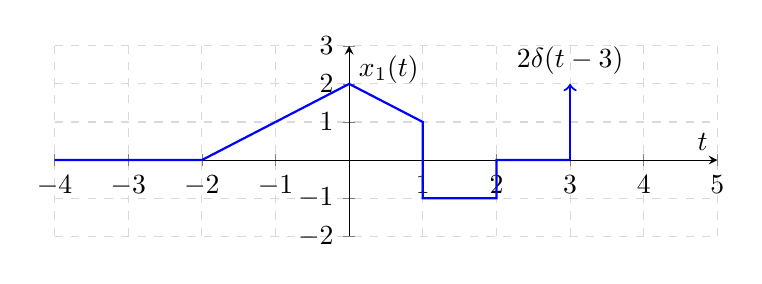
\begin{tikzpicture}
\begin{axis}[
	width=10cm,
	height=4cm,
    axis lines=middle,
    xlabel={$t$},
    ylabel={$x_1(t)$},
    xmin=-4, xmax=5,
    ymin=-2, ymax=3,
    xtick={-4,-3,-2,-1,0,1,2,3,4,5},
    ytick={-2,-1,0,1,2,3},
    grid=both,
    grid style={dashed, gray!30},
    samples=100
]
    \addplot[thick, blue] coordinates {(-4,0) (-2,0) (0,2) (1,1) (1,-1) (2,-1) (2,0) (3, 0)};
      
    % Impulse at t = 3 with weight 2
    \draw[->, thick, blue] (axis cs:3,0) -- (axis cs:3,2);
    \node[above] at (axis cs:3,2) {$2\delta(t-3)$};

\end{axis}
\end{tikzpicture}
\caption{A plot of $x_1(t)$}
\label{fig:x1}
\end{figure}

\begin{figure}[htbp]
\centering
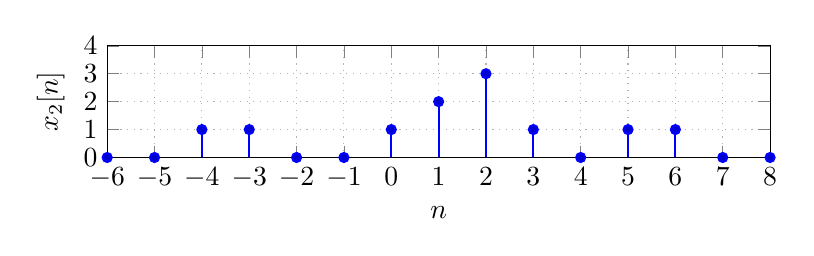
\begin{tikzpicture}
\begin{axis}[
    width=10cm,
    height=3cm,
    xlabel={$n$},
    ylabel={$x_2[n]$},
    xmin=-6, xmax=8,
    ymin=0, ymax=4,
    xtick={-6,-5,-4,-3,-2,-1,0,1,2,3,4,5,6,7,8},
    ytick={0,1,2,3,4},
    grid=both,
    grid style={dotted, gray!60},
    % Stem plot styling
    every axis plot/.append style={
        ycomb,
        black,
        thick,
        mark=*,
        mark options={fill=black, scale=0.8}
    }
]

\addplot coordinates {
    (-6,0) (-5,0) (-4,1) (-3,1) (-2,0) (-1,0) 
    (0,1)  (1,2)  (2,3)  (3,1)  (4,0)  (5,1)  
    (6,1)  (7,0)  (8,0)
};

\end{axis}
\end{tikzpicture}
\caption{A plot of $x_2[n]$}
\label{fig:x2n}
\end{figure}

\section*{\underline{Question 5: [10 Points]}}

Consider the signal $x[n]$ depicted as below

\begin{figure}[htbp]
\centering
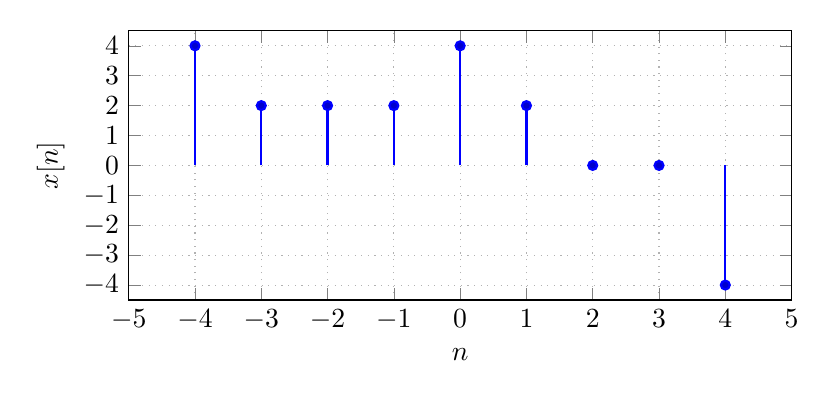
\begin{tikzpicture}
\begin{axis}[
    width=10cm,
    height=5cm,
    xlabel={$n$},
    ylabel={$x[n]$},
    xmin=-5, xmax=5,
    ymin=-4.5, ymax=4.5,
    xtick={-5,-4,-3,-2,-1,0,1,2,3,4,5},
    ytick={-4,-3,-2,-1,0,1,2,3,4},
    grid=both,
    grid style={dotted, gray!60},
    % Stem plot styling
    every axis plot/.append style={
        ycomb,
        black,
        thick,
        mark=*,
        mark options={fill=black, scale=0.8}
    }
]

\addplot coordinates {
    (-4,4) (-3,2) (-2,2) (-1,2) (0,4) (1,2)  (2,0)  (3,0)  (4,-4) 
};

\end{axis}
\end{tikzpicture}
\caption{(Note that $x[n]=0$ for all $|n| \geq5$))}
\label{fig:x2n}
\end{figure}

\begin{enumerate}
	\item Is $x[n]$ even, odd or neither?
	\item The decomposition into its even and odd componets $x[n] =x_\text{even}[n] + x_\text{odd}[n]$ is given by: $x_\text{even}[n] = \frac{x[n] +x[-n]}{2}$ and $x_\text{odd}[n] = \frac{x[n] - x[-n]}{2}$. Give the plots of $x_\text{even}[n]$ and $x_\text{odd}[n]$.
\end{enumerate}

\end{document}
